%!TEX root = ../template.tex
%%%%%%%%%%%%%%%%%%%%%%%%%%%%%%%%%%%%%%%%%%%%%%%%%%%%%%%%%%%%%%%%%%%%
%% chapter4.tex
%% NOVA thesis document file
%%
%% Chapter with lots of dummy text
%%%%%%%%%%%%%%%%%%%%%%%%%%%%%%%%%%%%%%%%%%%%%%%%%%%%%%%%%%%%%%%%%%%%

\typeout{NT FILE chapter4.tex}%

\chapter{Proposed Work}
\label{cha:proposed_work}

This chapter aims to outline the approach that will be used to achieve the project objectives defined in Chapter \ref{cha:introduction} while providing the prior work in the various areas relevant to this study.

\section{Requirements}

This section describes the requirements and functionalities to be developed during this dissertation. These are categorized into the following areas: Interactive Map, \gls{3D} Model Interaction, Repository, and \gls{VR} Integration.

\subsection*{Interactive Map}
\begin{itemize}
    \item \textbf{Map Zoom \& Navigation:} Users can pan, zoom, and explore different locations.
    \item \textbf{Perspective Switching:} Toggle between top-down and profile views for better spatial understanding.
    \item \textbf{Geospatial Data Integration:} Include \gls{GIS} layers combining excavation findings, and overlay a \textit{.tif} map illustration with some immersive interaction.
    \item \textbf{Layer Toggle:} Toggle visibility of layers, such as excavation campaigns or glass antiquities.
    \item \textbf{Parallel Objects:} Link parallel excavation findings/museums, possibly integrating them in the object pop-up ion the map.
\end{itemize}

\subsection*{\gls{3D} Models \& Interaction}
\begin{itemize}
    \item \textbf{Artifact Interaction:} Allows users to virtually manipulate (rotate, zoom etc) the glass artifact models, as well as apply different textures.
    \item \textbf{Contextual Overlay:} Display descriptive metadata about the artifact, such as its origin, period, and historical usage.
    \item \textbf{Reconstructed Models:} Showcase how artifacts would look originally(having in consideration characteristics such as: colourless glass, archeological drawings and symmetry). However, due to time constraints, the reconstruction funcionality may not be completed.
    \item \textbf{3D Models Integration:} The user can zoom the map to visualize the perspective of a specific \gls{3D} model.
    %select a position to visualize the perspective of their 3D model.
\end{itemize}

\subsection*{Repository}
\begin{itemize}
    \item \textbf{Document Upload/Download:} Allow contributors to upload images, videos or excavation reports of the archeological intervention.
    \item \textbf{Search and Filter Features:} Users can search and filter based on some fields, such as time period, shape, and provenance.
    \item \textbf{Digital Preservation:} The usage of open, and standard formats to ensure a long-term resource access.
\end{itemize}


\subsection*{\gls{VR} Integration}
\begin{itemize}
    \item \textbf{Immersive Experience:} \gls{VR} allows users to immerse in a virtual tomb visit, enabling interaction with glass relics.
    \item \textbf{Device Accessibility:} Primarily user-friendly and enabling haptic interaction, while supporting \gls{AR} glasses as an emerging display option.
    \item \textbf{Localization \& Wayfinding:} 
    \begin{itemize}
        \item \textbf{\gls{POI}:} Use colors, text, visual markers, or direction arrows to emphasize and guide users to historically significant locations.
    \end{itemize}
   % \item \textbf{Multilingual Support:} Provide language options to ensure accessibility for an international audience.
\end{itemize}



\section{Development Technologies and Tools}
\label{sec:technologies}

The following section focuses on the technologies and tools that will be used in the implementation of this project. These include frontend, backend, database, and \gls{3D} development tools.

\subsection{Frontend Technologies}
\label{sec:frontend}

JavaScript is a programming language mostly used to control interactive behavior in web
pages. To make a map interactive, most websites automatically send JavaScript code to the browser.~\cite{ajayi2024utilizing} In this project, this language will be used for client-side web development and to integrate frameworks that enhance map interactivity.

Leaflet\footnote{\url{https://leafletjs.com/}} is an open-source JavaScript library that facilitates the creation of mobile-friendly interactive maps. It offers a wide array of plugins that improve usability and simplify application development.
Leaflet will be employed in this thesis to integrate interactive map features and create an intuitive user interface.

Other alternatives for web development frameworks used for map rendering and interaction include OpenLayers\footnote{\url{https://openlayers.org/}}, which enables the integration of dynamic maps into web pages and can display map tiles, vector data, and markers loaded from any source.
Another powerful tool is the Google Maps API\footnote{\url{https://developers.google.com/maps}}, which allows developers to embed Google Maps functionalities directly into both web and mobile applications.
Additionally, Mapbox\footnote{\url{https://www.mapbox.com/}} and \gls{OSM}\footnote{\url{https://www.openstreetmap.org/}} provide online mapping solutions. While \gls{OSM} is open-source, offering greater flexibility and customization, and is maintained and updated by the community, Mapbox and Google Maps API have usage-based pricing plans.
For this dissertation, one of these technologies will be used to create an interactive map, complementing an existing illustration of the Troia site area, that includes the mausoleum under study. This will be supplemented with an open map, potentially sourced from \gls{OSM}\footnote{\url{https://www.openstreetmap.org/}}.
%REACT????

%Turf\footnote{\url{https://turfjs.org/}}
%Some popular options include 
%ArcGIS
%QGIS
%Other alternatives for web development
%notable
%Google Maps API provides extensive features such as map layers, markers, street view, and geocoding.
\subsection{Backend Technologies}
\label{sec:backend} 

The backend tecnologies selected for this thesis include the C\# programming language integration in Unity for scene interactions in the \gls{VE}.
Additionally, Node.js\footnote{\url{https://nodejs.org/}} software was choosen. Node.js is an open-source and cross-platform JavaScript runtime environment that enables developers to create servers, web applications, command-line tools, and automation programs.
This tool will be use to support the web server and to improve performance and scalibility when managing with repository data.


\subsection{Database Repository}
\label{sec:repos}

There are several alternatives for storage management systems, but the options are more limited when it comes to geographical
database systems.

For this project, organizing the data in a relational database is more appropriate due to its flexibility and consistency.
The most common databases for such applications include PostGIS, extension for PostgreSQL, MySQL\footnote{\url{https://www.mysql.com/}} and Oracle.
All three databases databases support spatial data types, allowing to store and manage geographic objects, representing them with points, lines, or polygons, and performing geospatial queries.
Among these, PostGIS is widely used for spatial data storage, geometry processing, and efficient geospatial querying.
Oracle supports advanced spatial features and 3D features but has a commercial license. On the other hand, MySQL is open-source and more suitable for small-to-medium-scale projects.

PostgreSQL database was chosen for this thesis because of its high performance and flexibility in managing spatial data. All geographic data, artifacts metadata, and excavation details will be stored within this system.


\subsection{Unity Engine}
\label{sec:unity_description} 

Unity is a cross-platform engine that provides a robust environment for developing \gls{2D} and \gls{3D} applications. 
Its component-based architecture simplifies \gls{3D} development by allowing developers to define object behaviors through scripts in \glspl{VE}.
Despite not being open-source, Unity offers a community forum and repositories where developers can access resources, and adapt them for their projects.
Additionally, the Unity Learn\footnote{\url{https://learn.unity.com/}} platform provides free tutorials, simplifying the learning process.

Unity will be a fundamental technology for supporting the \gls{VR} development of this project. Its integration enables users an immersive experience by visualizing several \gls{3D} data types, including excavation and glass artifacts metadata. 


\subsection{Photogrammetry Tools}
\label{sec:photogrammetry_tool} 

The software that will be used to process digital images and generate \gls{3D} object models is \textit{Agisoft Metashape}\footnote{\url{https://www.agisoft.com/}}.
This software performs photogrammetric processing of digital images to generate \gls{3D} spatial data, which can be applied in various fields such as \gls{GIS} applications, \gls{CH} documentation, visual effects production, and indirect measurements of objects of diverse scales. 
By stitching together photographs, \textit{Agisoft Metashape} captures the geometry, texture, and visual appearance of physical objects or environments.
Other alternatives for photogrammetry softwares are Pix4D, RealityCapture and DroneDeploy

There are some already built models of the artifacts provided by Troia archaeologists, there will be done a selection and evaluation of the greatest possibilities.


\section{System Architecture}
\label{sec:architecture}

This section includes an overview of the system architecture. The communication flow between the layers will be conducted by a REST \gls{API}.
REST \glspl{API} connect components in microservices architectures\footnote{{https://www.ibm.com/think/topics/rest-apis}}.
This service was selected due to its flexiblility and lightweight solution. 

\begin{figure}[h!]
    \centering
    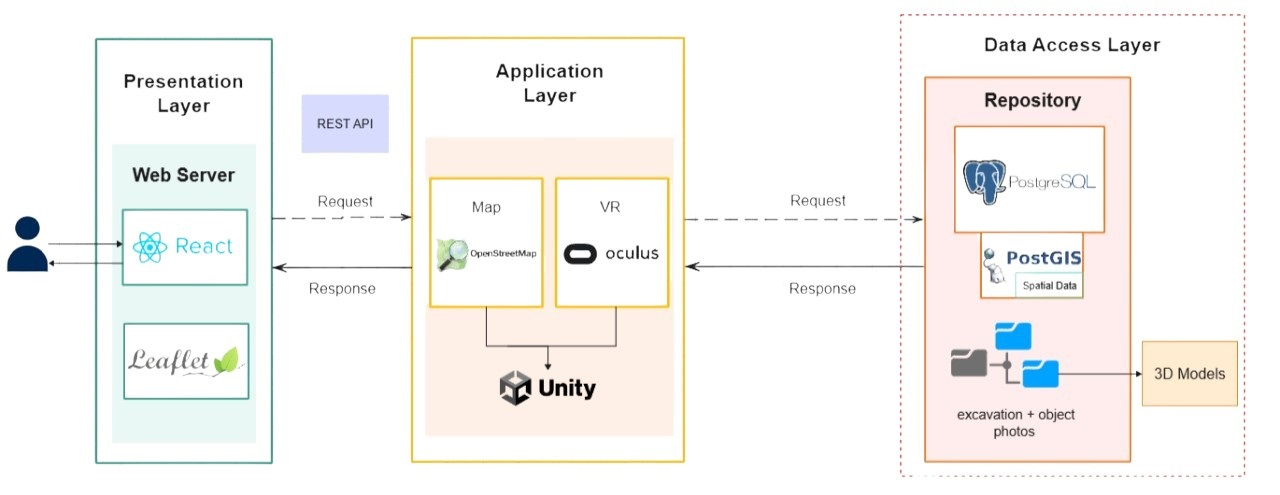
\includegraphics[width=1.0\linewidth]{System Architecture-Photoroom_Right}
    \caption{System Architecture Overview}
    \label{fig:architecture}
  \end{figure}
  \FloatBarrier


\section{Usability Tests}
\label{sec:usability_tests}

The Usability Tests will be conducted both remotely and presencially throughout the implementation process, concretely the \gls{HMD} interactions will be done in person.
Investigators from \gls{VICARTE} will participate in these tests with valuable feedback to improve the platform, while providing input on their archeology necessities. Their collaboration will contribute to a more useful, accurate, and user-friendly platform.

\section{Previous Work}
\label{sec:previous_work}

During my internship, I developed a platform using React and TailwindCSS for the web layer, with C\# and ASP.NET for the application layer, and MongoDB\footnote{\url{https://www.mongodb.com/}} for data storage. Communication between these three components was handled through direct requests to the web server, which forwarded \gls{CRUD} operations and interacted with the database.  
Additionally, the Database Systems and Cloud Computation Systems master's course provided me with hands-on experience in various storage methodologies and introduced me to different technologies and alternative solutions for data management.

This section explains the various experiments carried out during the preparation phase.

\subsection{Geographic Information System}
\label{sec:gis_previous} 

To deepen my expertise in \gls{GIS}, I enrolled in the master's course \textit{Web Geográfica}, taught by my thesis adviser, Armanda Rodrigues. During this course, I developed a Web \gls{3D} application designed to provide an interactive map for visualizing and analyzing demographic data, key infrastructure locations, and other notable European datasets. Although this project did not focus on archaeological data, it introduced me to and enriched my understanding of GIS concepts, map interaction, and geospatial analysis while exposing me to new technologies.

% The application leveraged PostGIS\footnote{https://postgis.net/}, a PostgreSQL extension, which is widely used for spatial data storage, geometry processing, and querying geospatial data efficiently.
% Additionally, used frameworks like Leaflet\footnote{https://leafletjs.com/}, an open-source JavaScript library that facilitates the creation of mobile-friendly interactive maps. Leaflet offers a wide array of plugins that improve the usability and simplicity of the application. For the base map, \gls{OSM}\footnote{https://www.openstreetmap.org/} was integrated, offering a customizable and versatile visualization. This project serves as a preparatory stage for my thesis, specifically for the \gls{GIS} component, in which I will develop an interactive map of the Tróia site.

The application leveraged PostGIS, a PostgreSQL extension to support spatial queries.
Additionally, frameworks like Leaflet were used for map rendering, visualization and user interaction. For the base map, \gls{OSM} was integrated, offering a customizable and versatile visualization. This project serves as a preparatory stage for my thesis, specifically for the \gls{GIS} component, in which I will develop an interactive map of the Troia site.

\section{Data Structure Proposal}
\label{sec:data_strucutre}

A data structure has been proposed and analysed for artifacts storage management.  
It incorporates the key characteristics of each object to ensure structured organization and availability.


\begin{figure}[h]
    \centering
    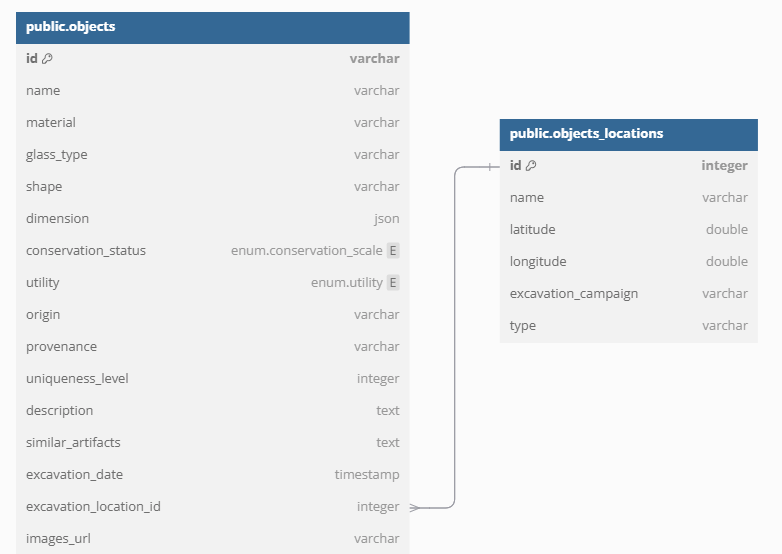
\includegraphics[width=0.7\textwidth]{data_structure}
    \caption{Proposed Data Structure for Managing Artifacts Data.}
    \label{fig:data_strucutre}
\end{figure}


\subsection{Photogrammetry}
\label{sec:photogrammetry_previous} 

A photogrammetric simulation was conducted using the \textit{Agisoft Metashape} environment. A total of 143 images were collected during the excavation campaign by the restoration department of NOVA, for analysis. 
Based on these images, a \gls{3D} model was generated and subsequently imported into the \textit{Sketchfab} viewer for intuitive interaction.
Within the grave where the deceased was buried, three open triangular areas were identified, containing the precious artifacts of the defunct, as shown in Figure~\ref{fig:model3} below.

\begin{figure}[h]
    \centering
    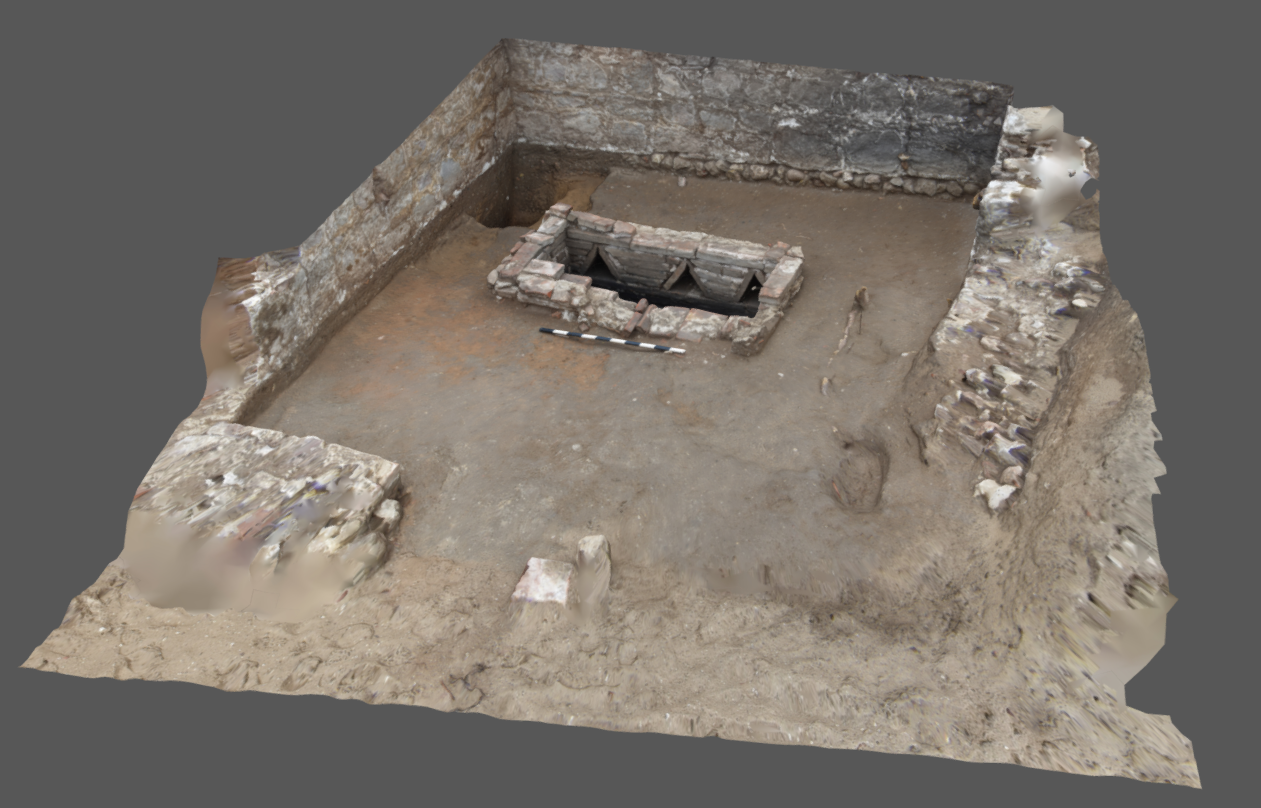
\includegraphics[width=0.7\textwidth]{model3}
    \caption{\gls{3D} Model Imported into Sketchfab for Visualization.}
    \label{fig:model3}
\end{figure}


\subsection{Unity}
\label{sec:unity} 

To reproduce the visualization of the \gls{3D} models on the map, a simulation was created in Unity, as presented in Figure \ref{fig:overlay}. The goal was to overlay the map with the \gls{3D} excavation model.
To achieve this, the illustrated map was placed as the ground surface, with the excavation model positioned above it. The ultimate objective is to apply this approach to the artifacts found within the three triangular areas of the grave.

This experiment simulates an intended interactive and dynamic experience, allowing users to explore the map and objects through interactive layers while using an \gls{HMD}.


\begin{figure}[h]
    \centering
    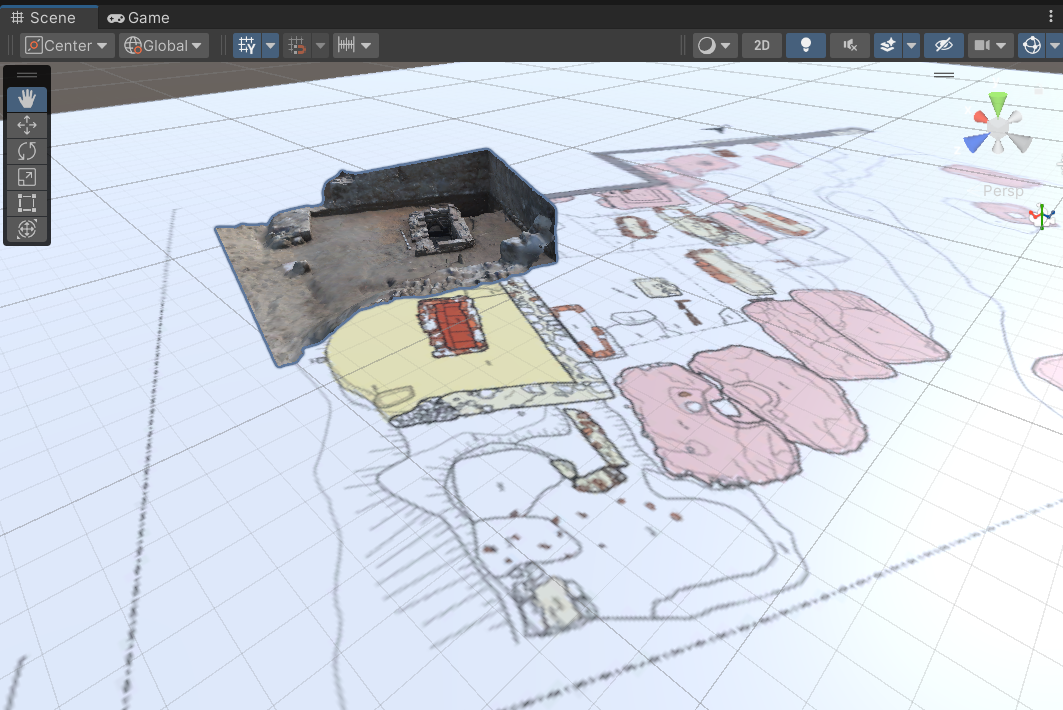
\includegraphics[width=0.7\textwidth]{overlay_test}
    \caption{Overlay \gls{3D} Excavation Model with a Map Representation.}
    \label{fig:overlay}
\end{figure}


%Insights from the Research Unit VICARTE